\begin{figure}[h!]
\centering
%
\begin{subfigure}{0.25\textwidth}
  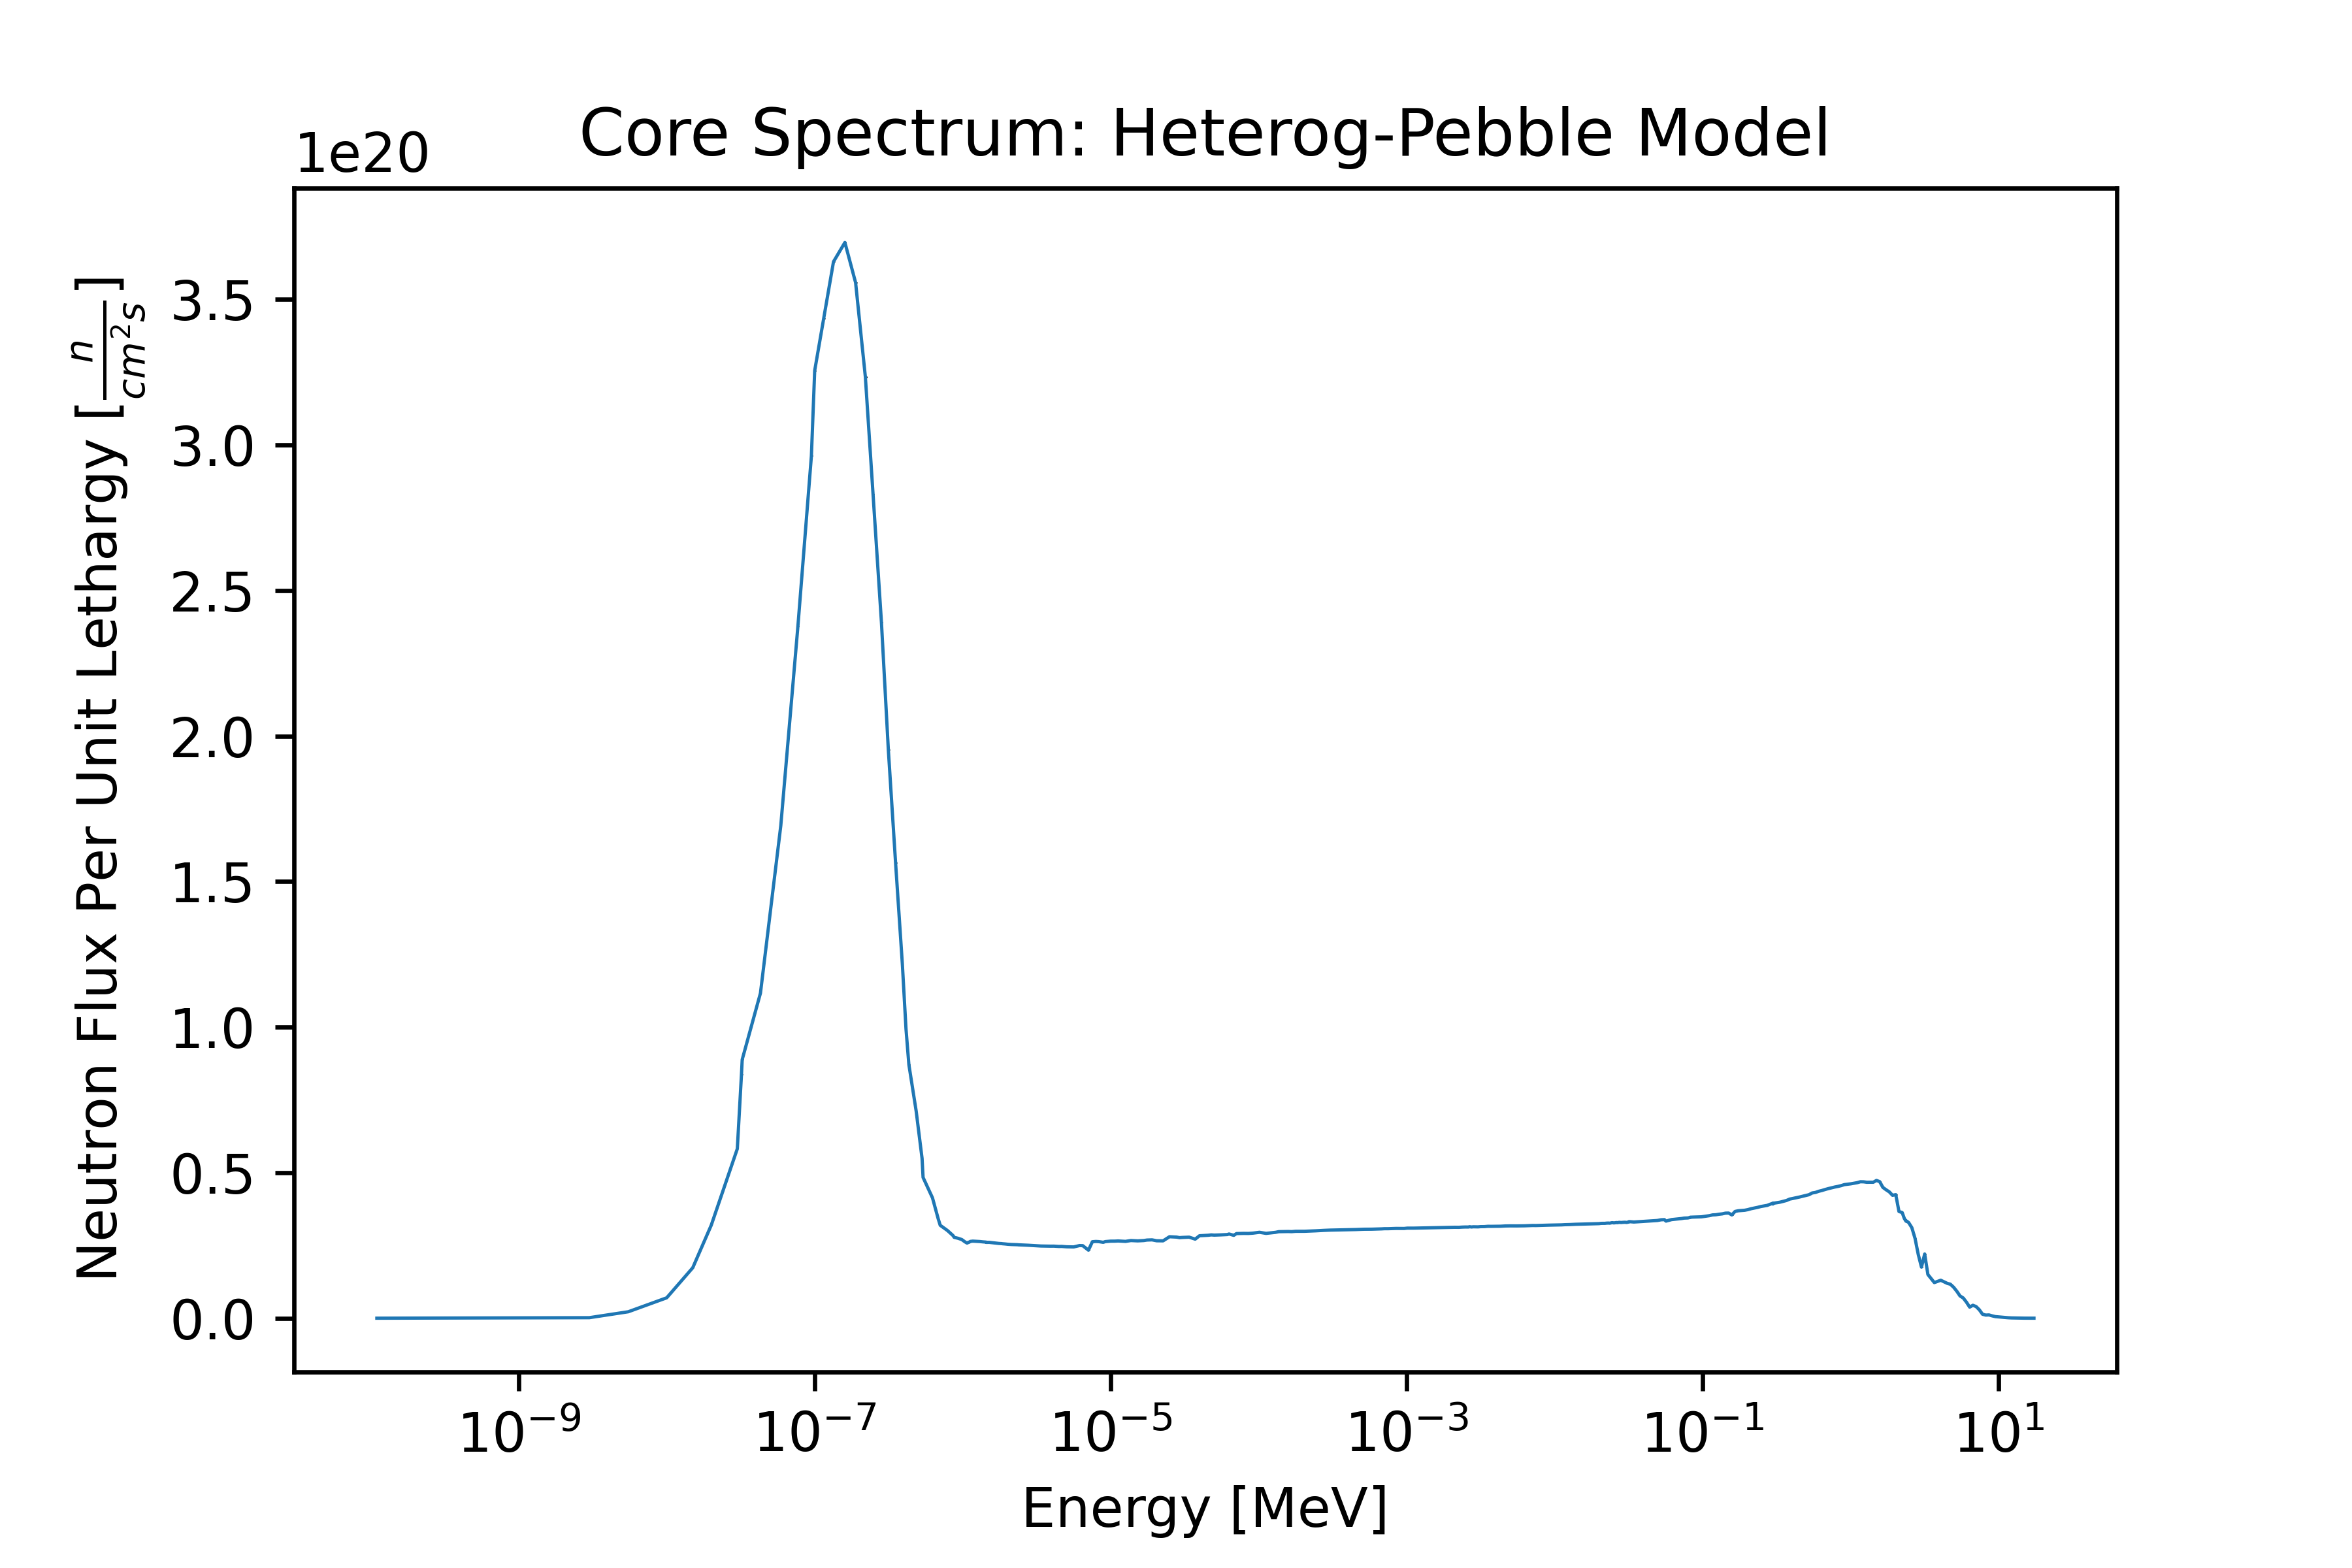
\includegraphics[width=0.95\linewidth]{figures/core_spec_het}
  \caption{Core Spectrum}
  \label{fig:het-core}
\end{subfigure}%
%
\begin{subfigure}{0.25\textwidth}
  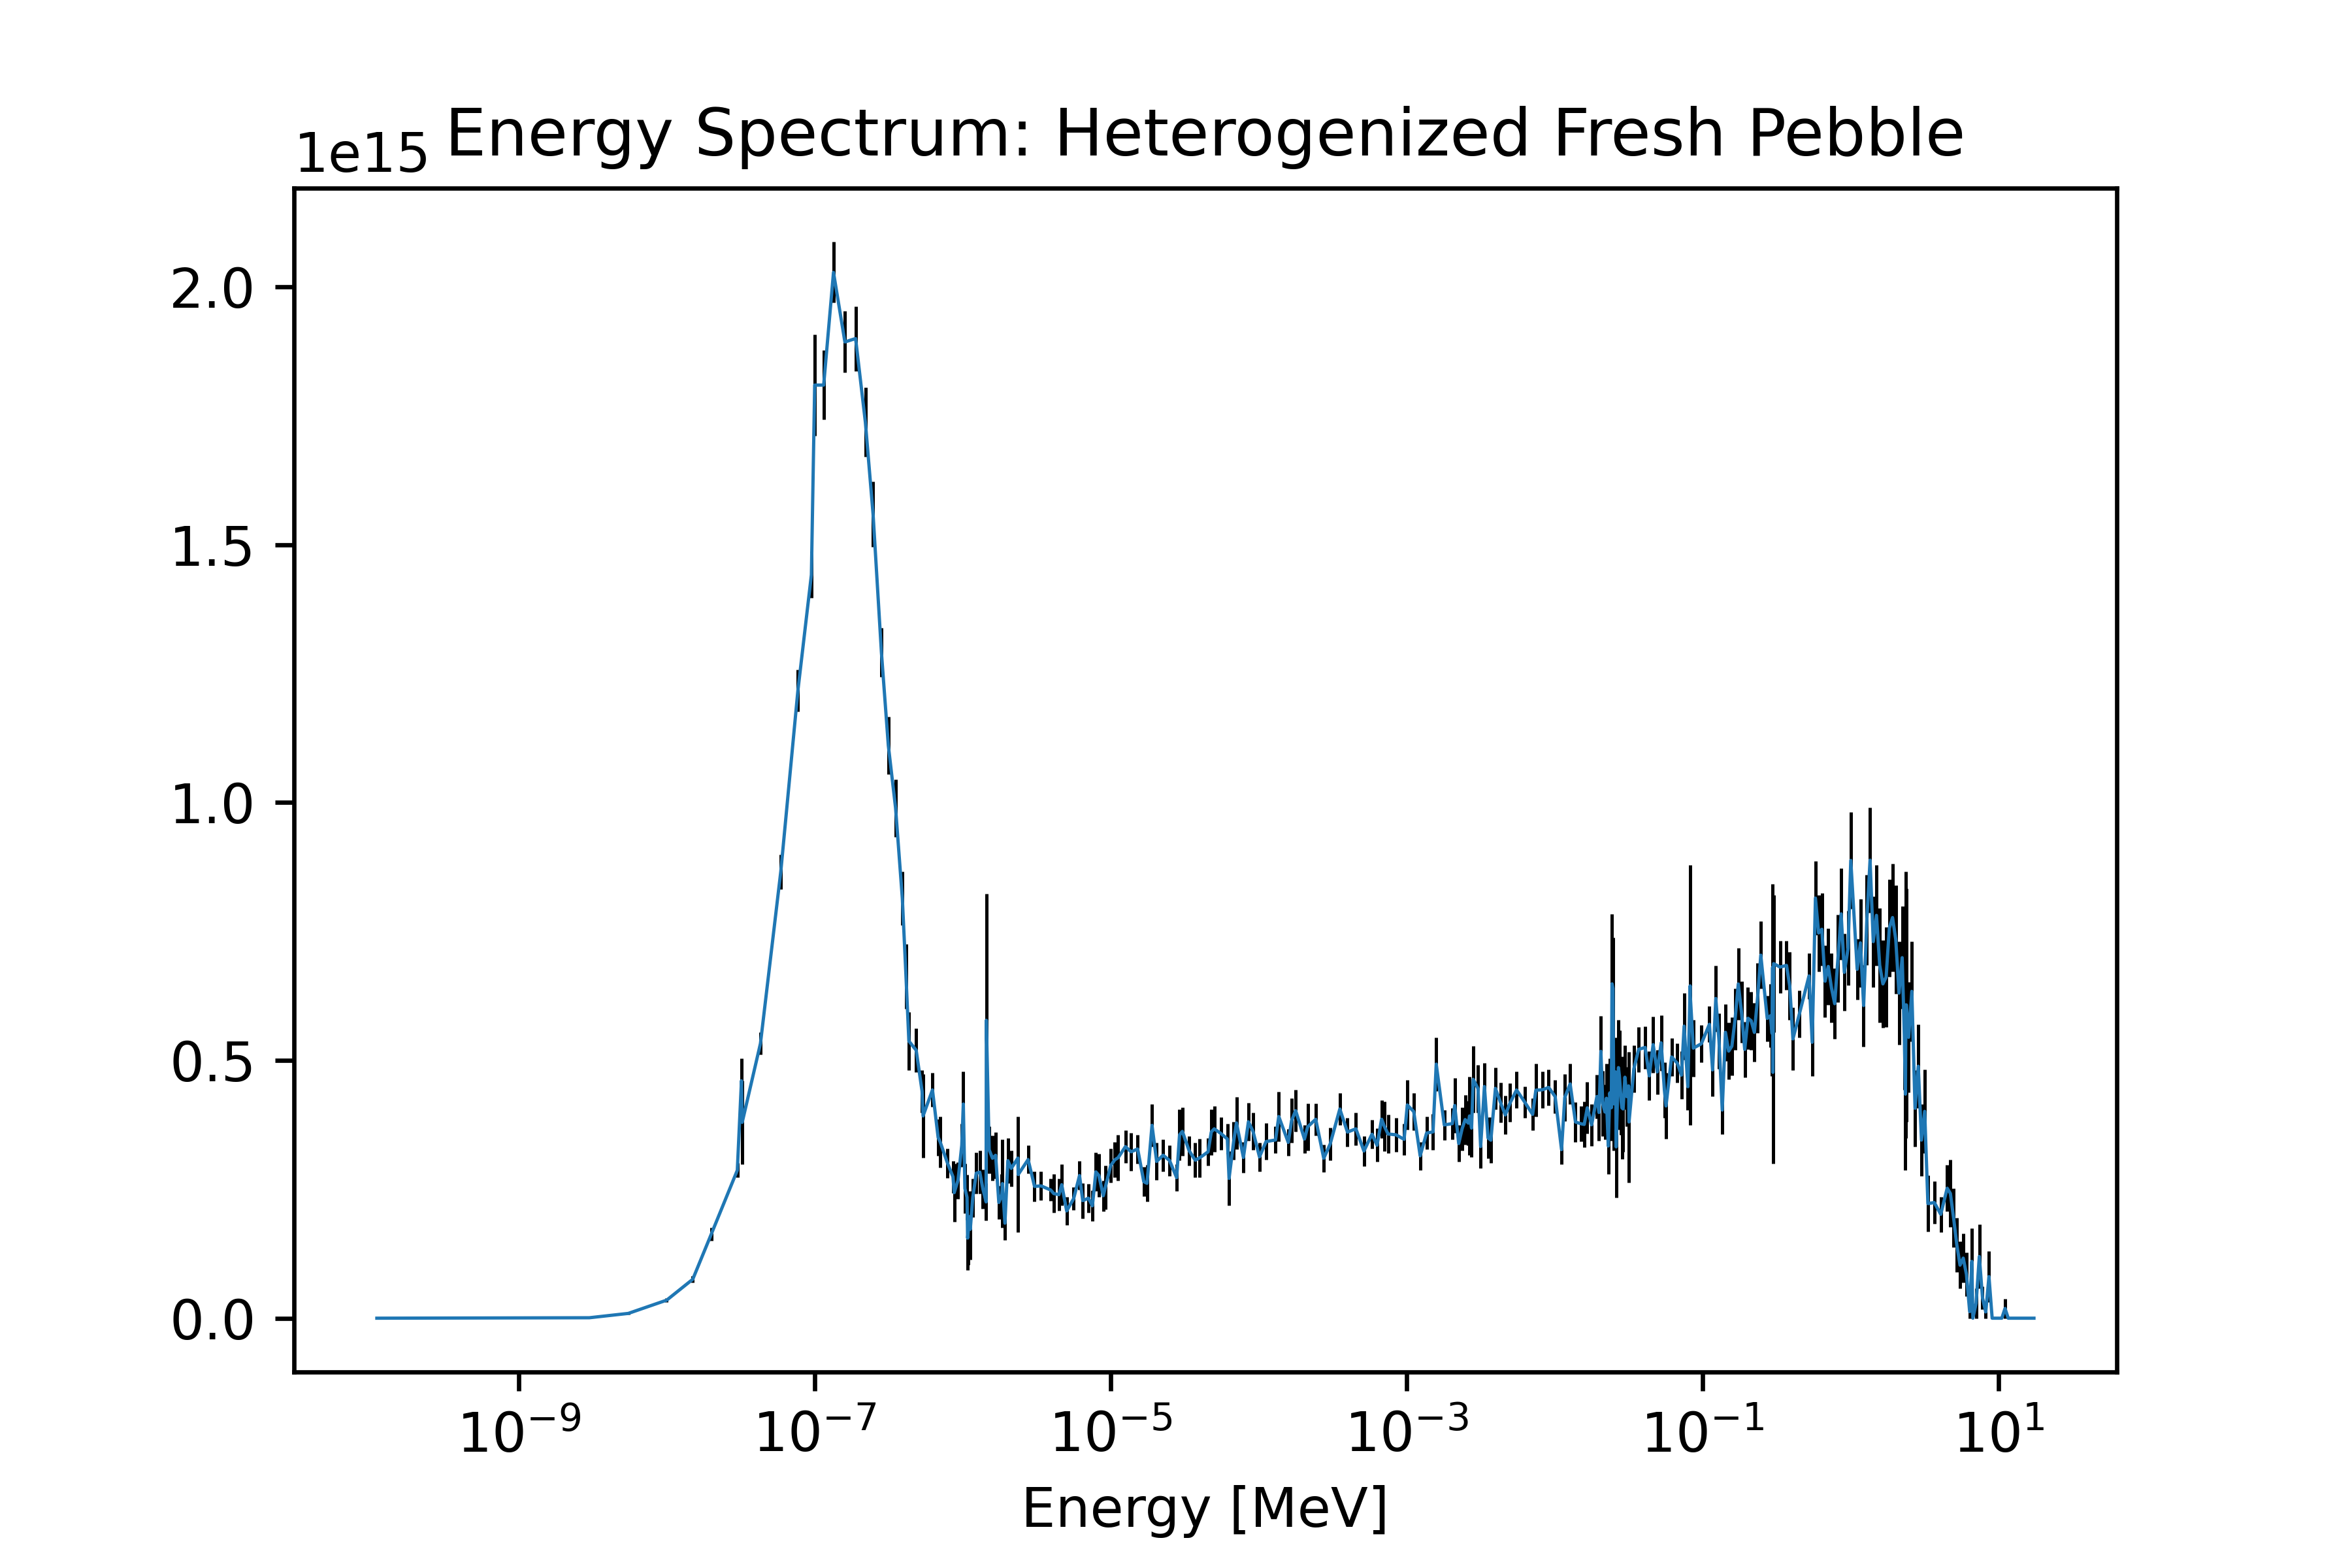
\includegraphics[width=0.95\linewidth]{figures/fresh_spec_het}
  \caption{Fresh Pebble Spectrum}
  \label{fig:het-fresh}
\end{subfigure}%
%
\begin{subfigure}{0.25\textwidth}
  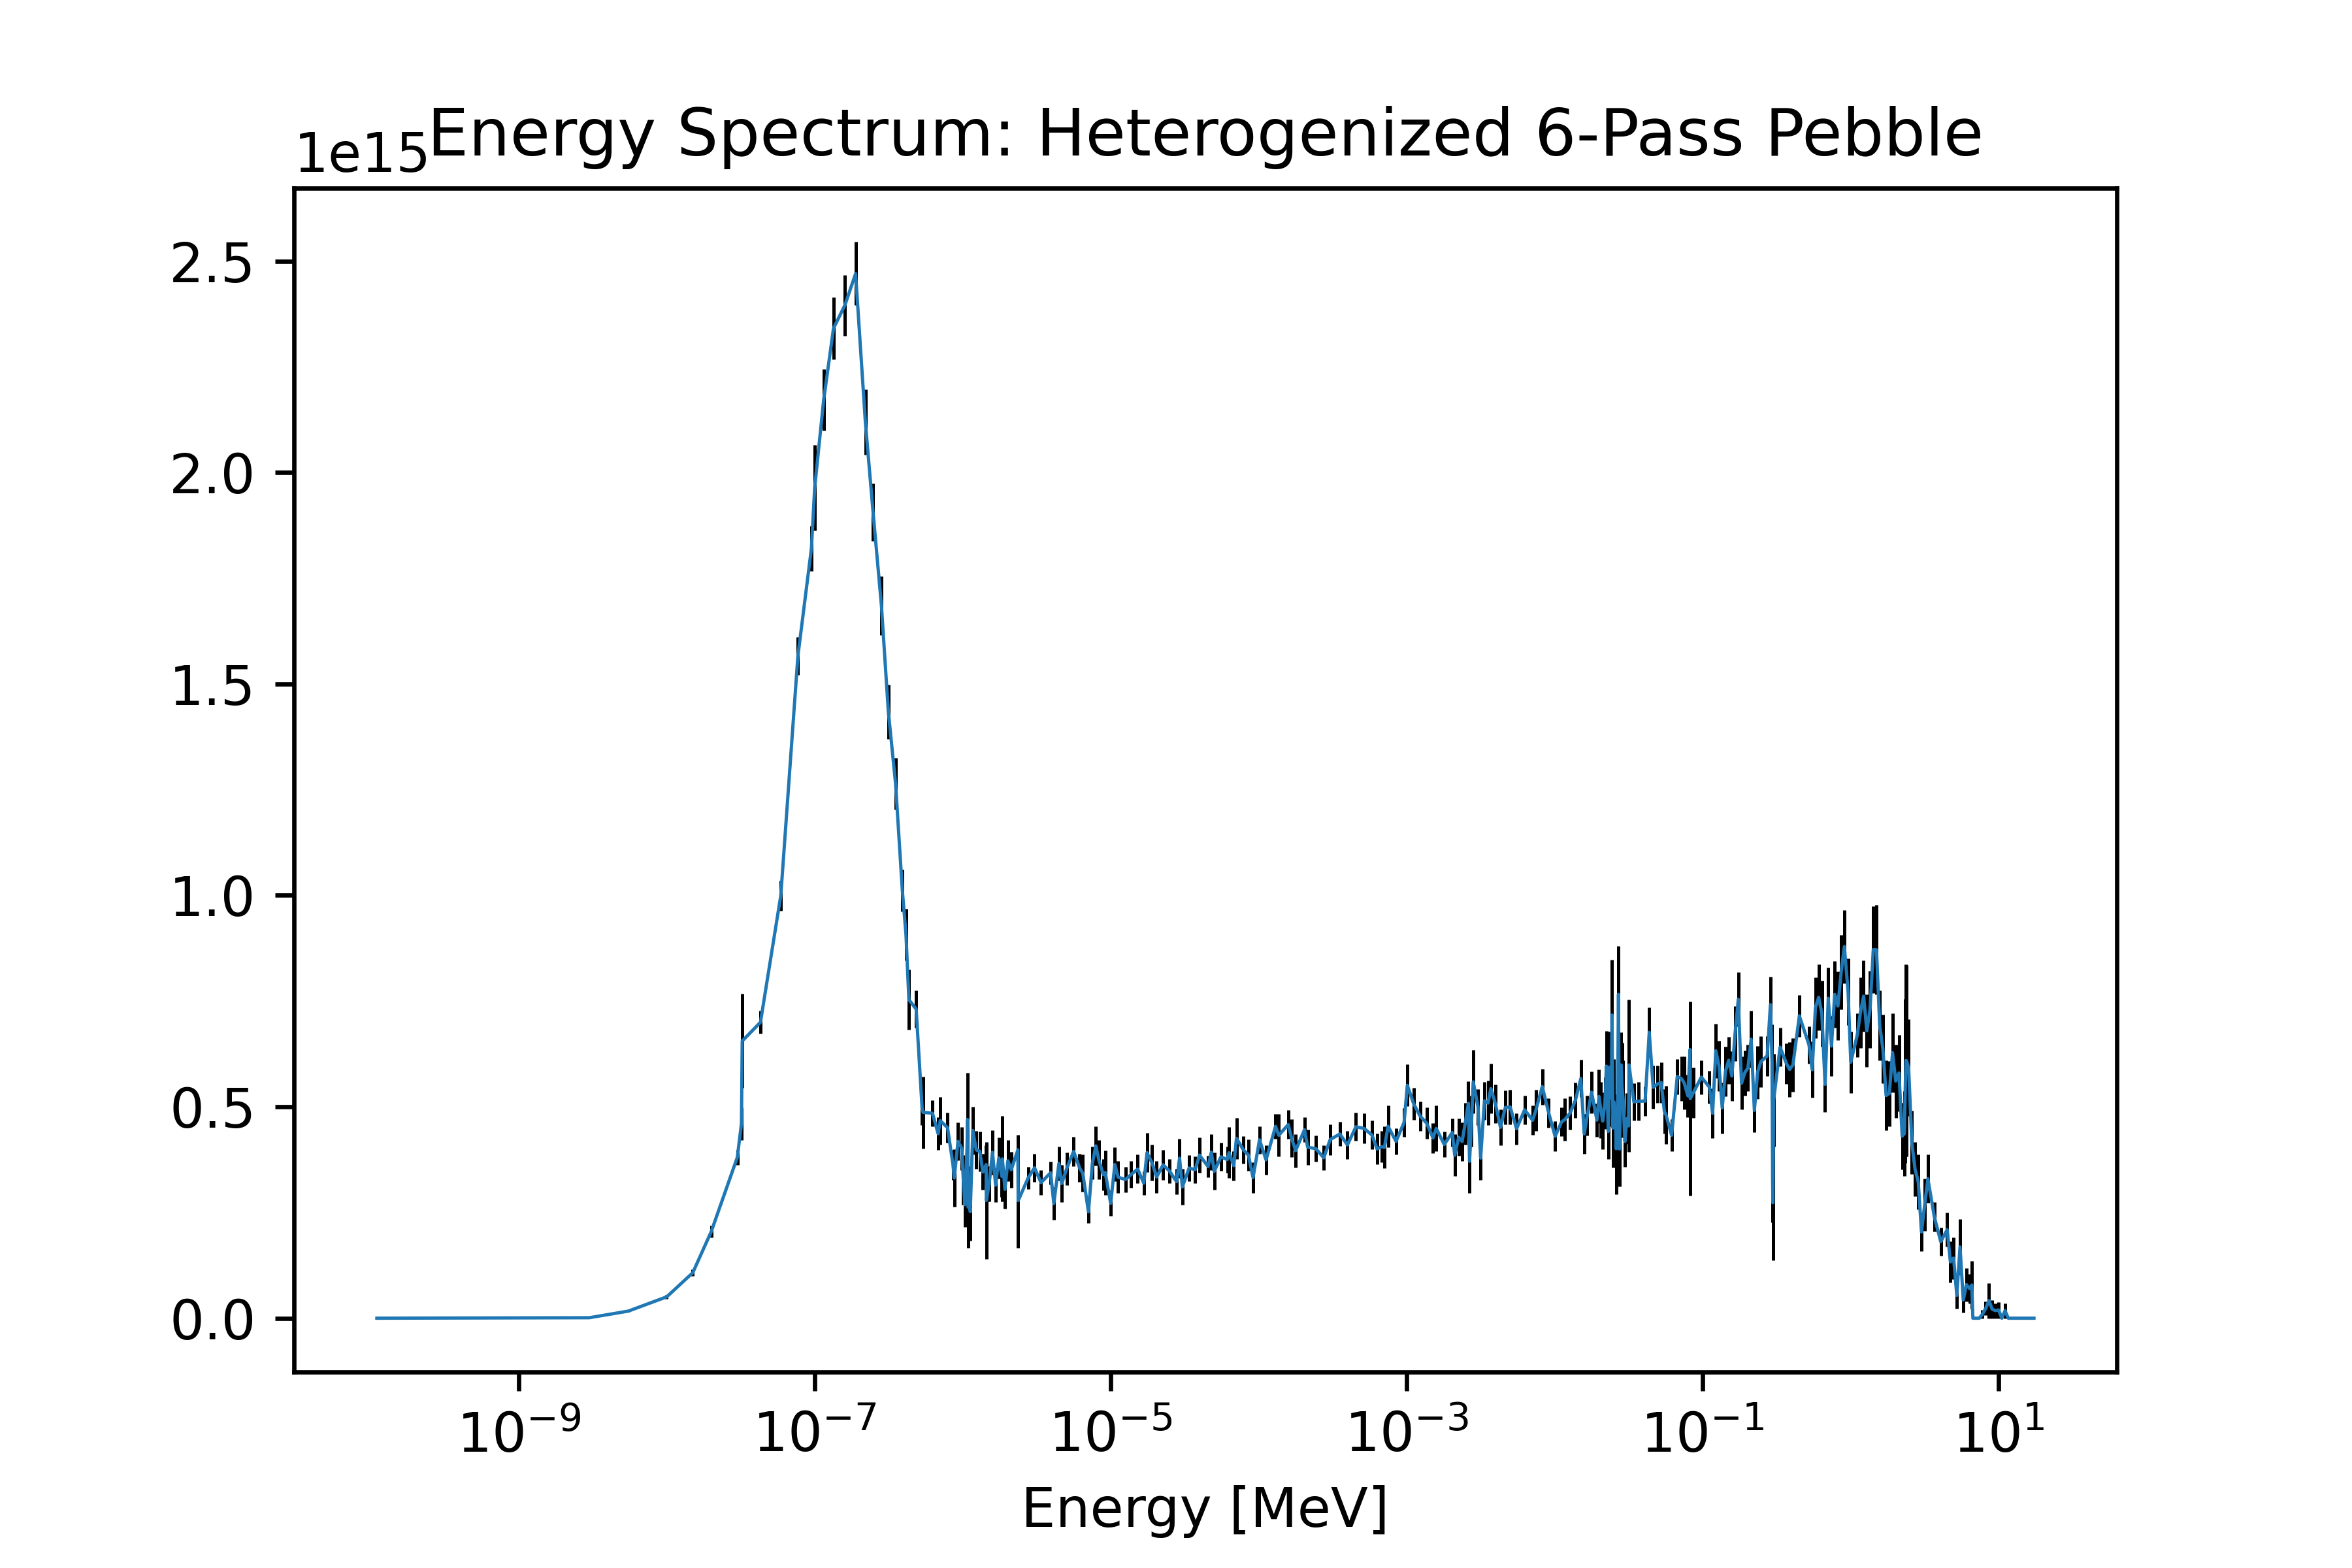
\includegraphics[width=0.95\linewidth]{figures/6_spec_het}
  \caption{Six-Pass Pebble Spectrum}
  \label{fig:het-six}
\end{subfigure}%

\begin{subfigure}{0.25\textwidth}
  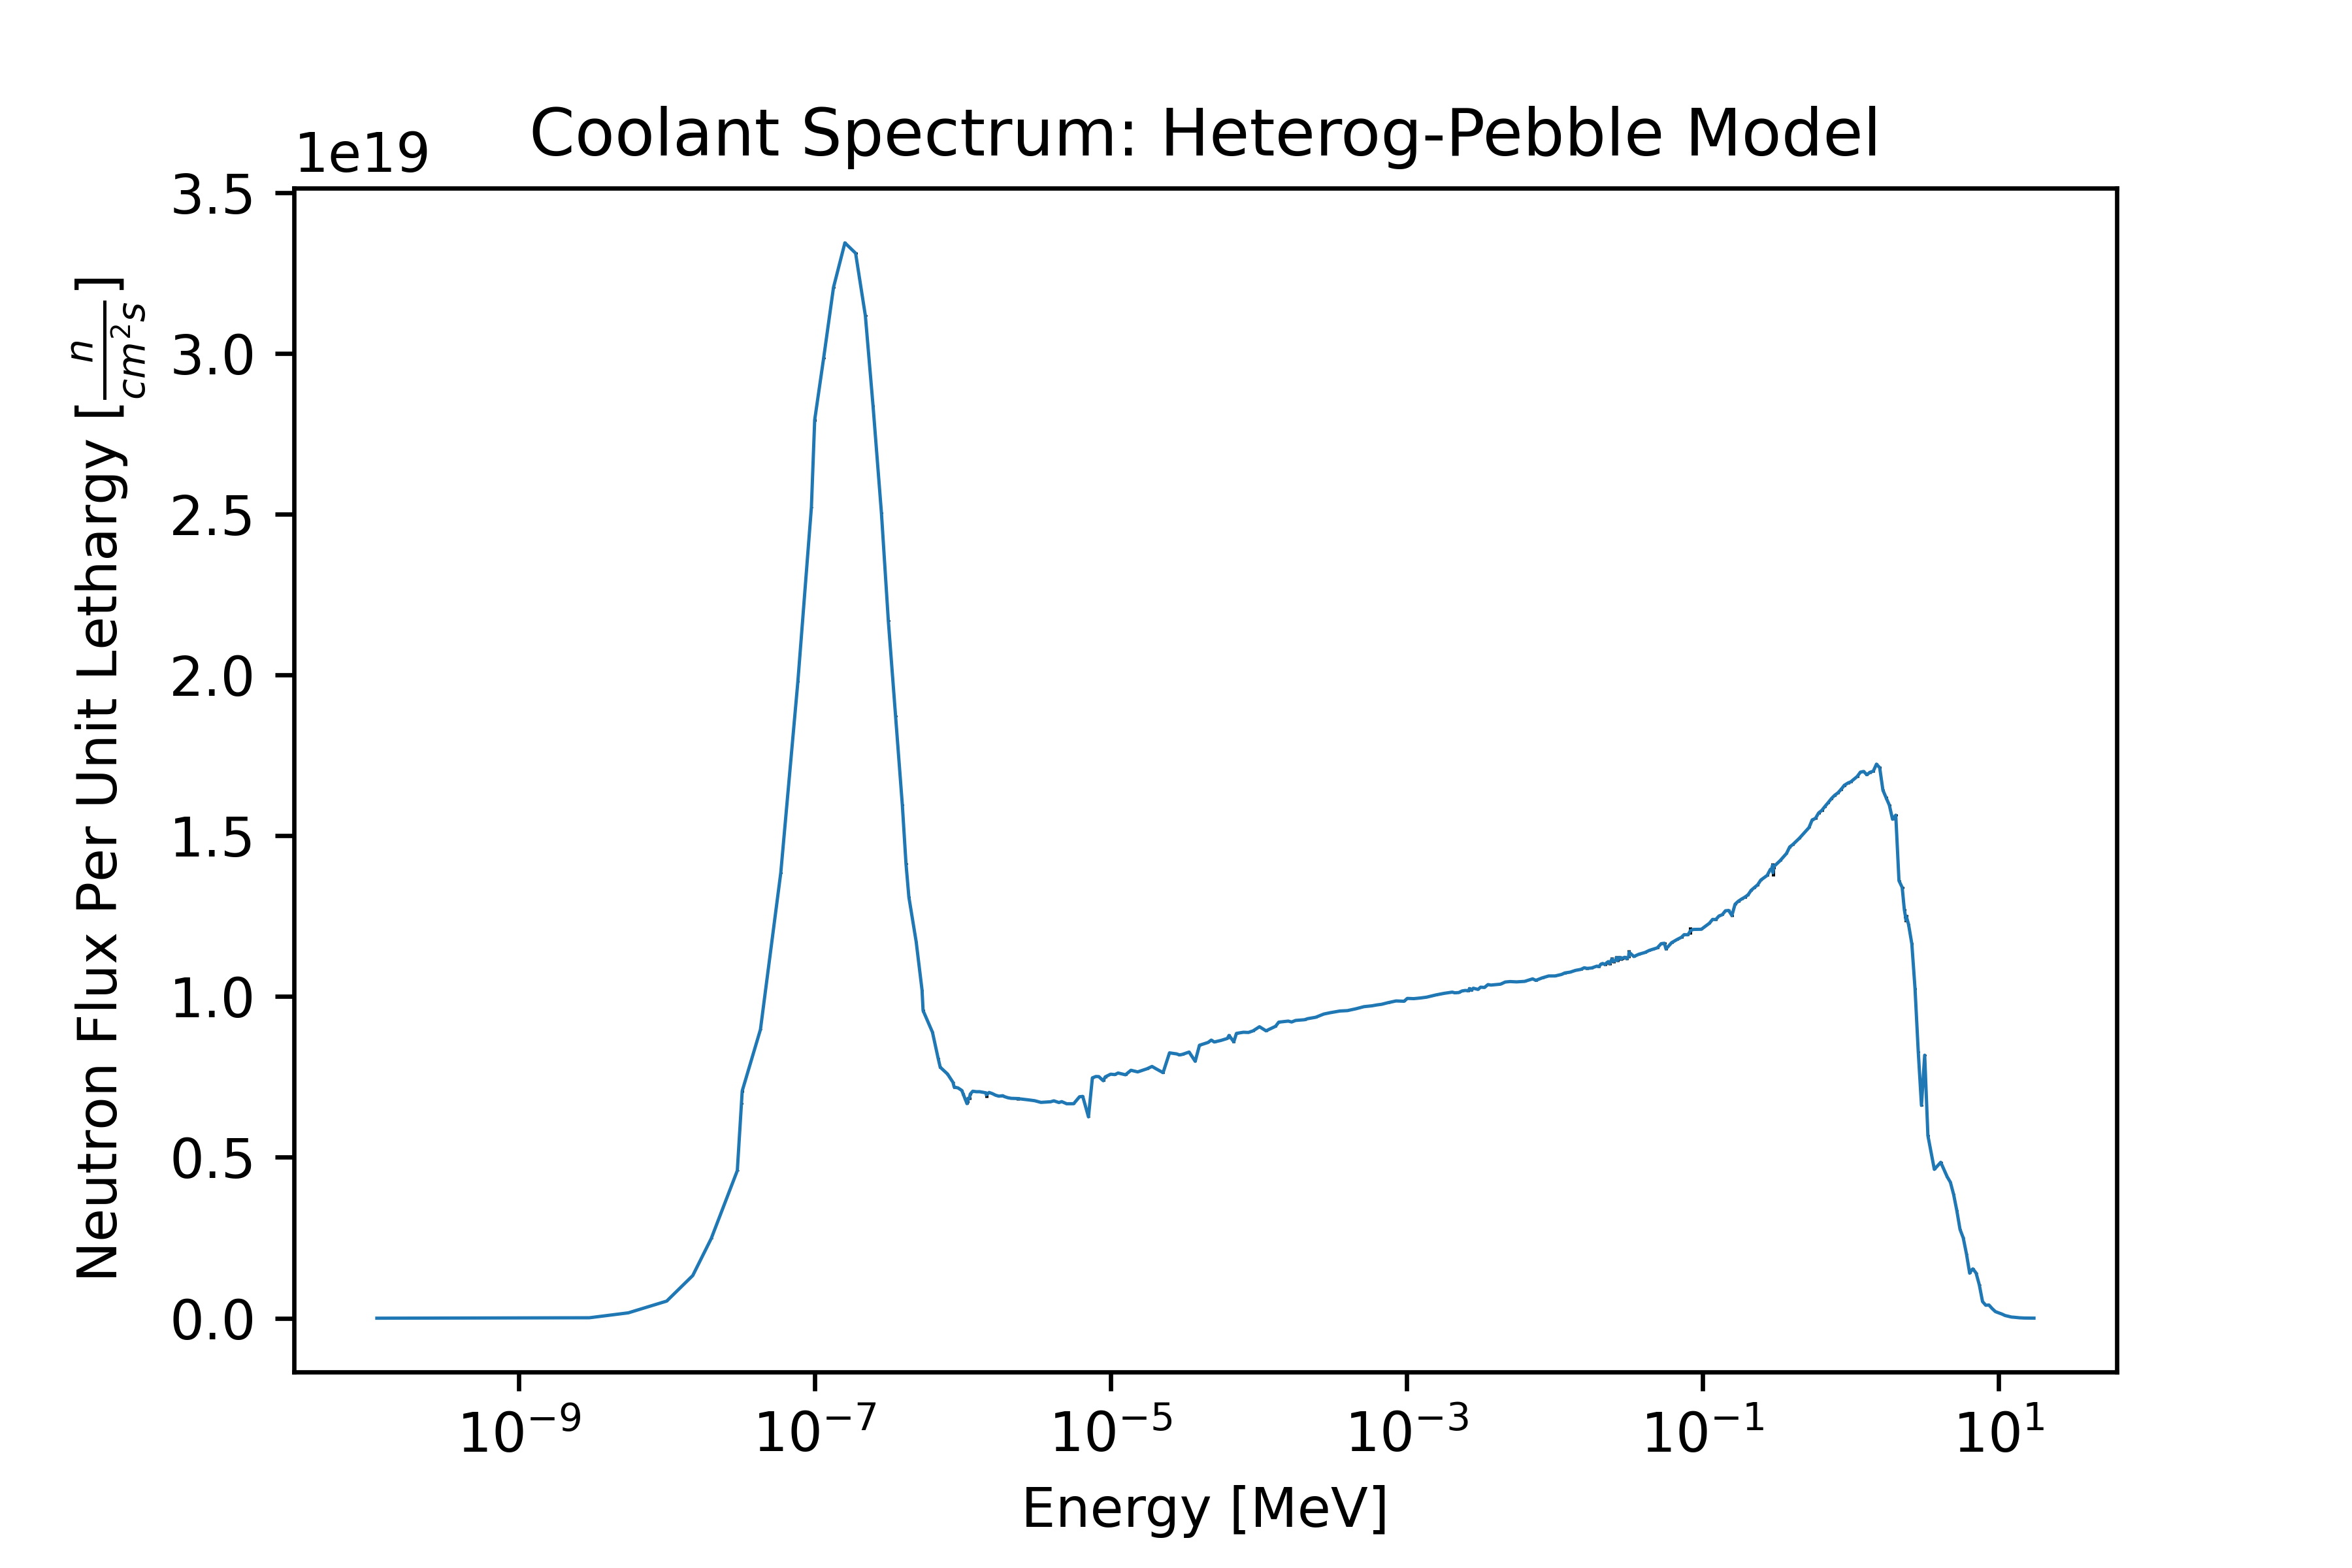
\includegraphics[width=0.95\linewidth]{figures/cool_spec_het}
  \caption{Coolant Spectrum}
  \label{fig:het-cool}
\end{subfigure}%
%
\begin{subfigure}{0.25\textwidth}
  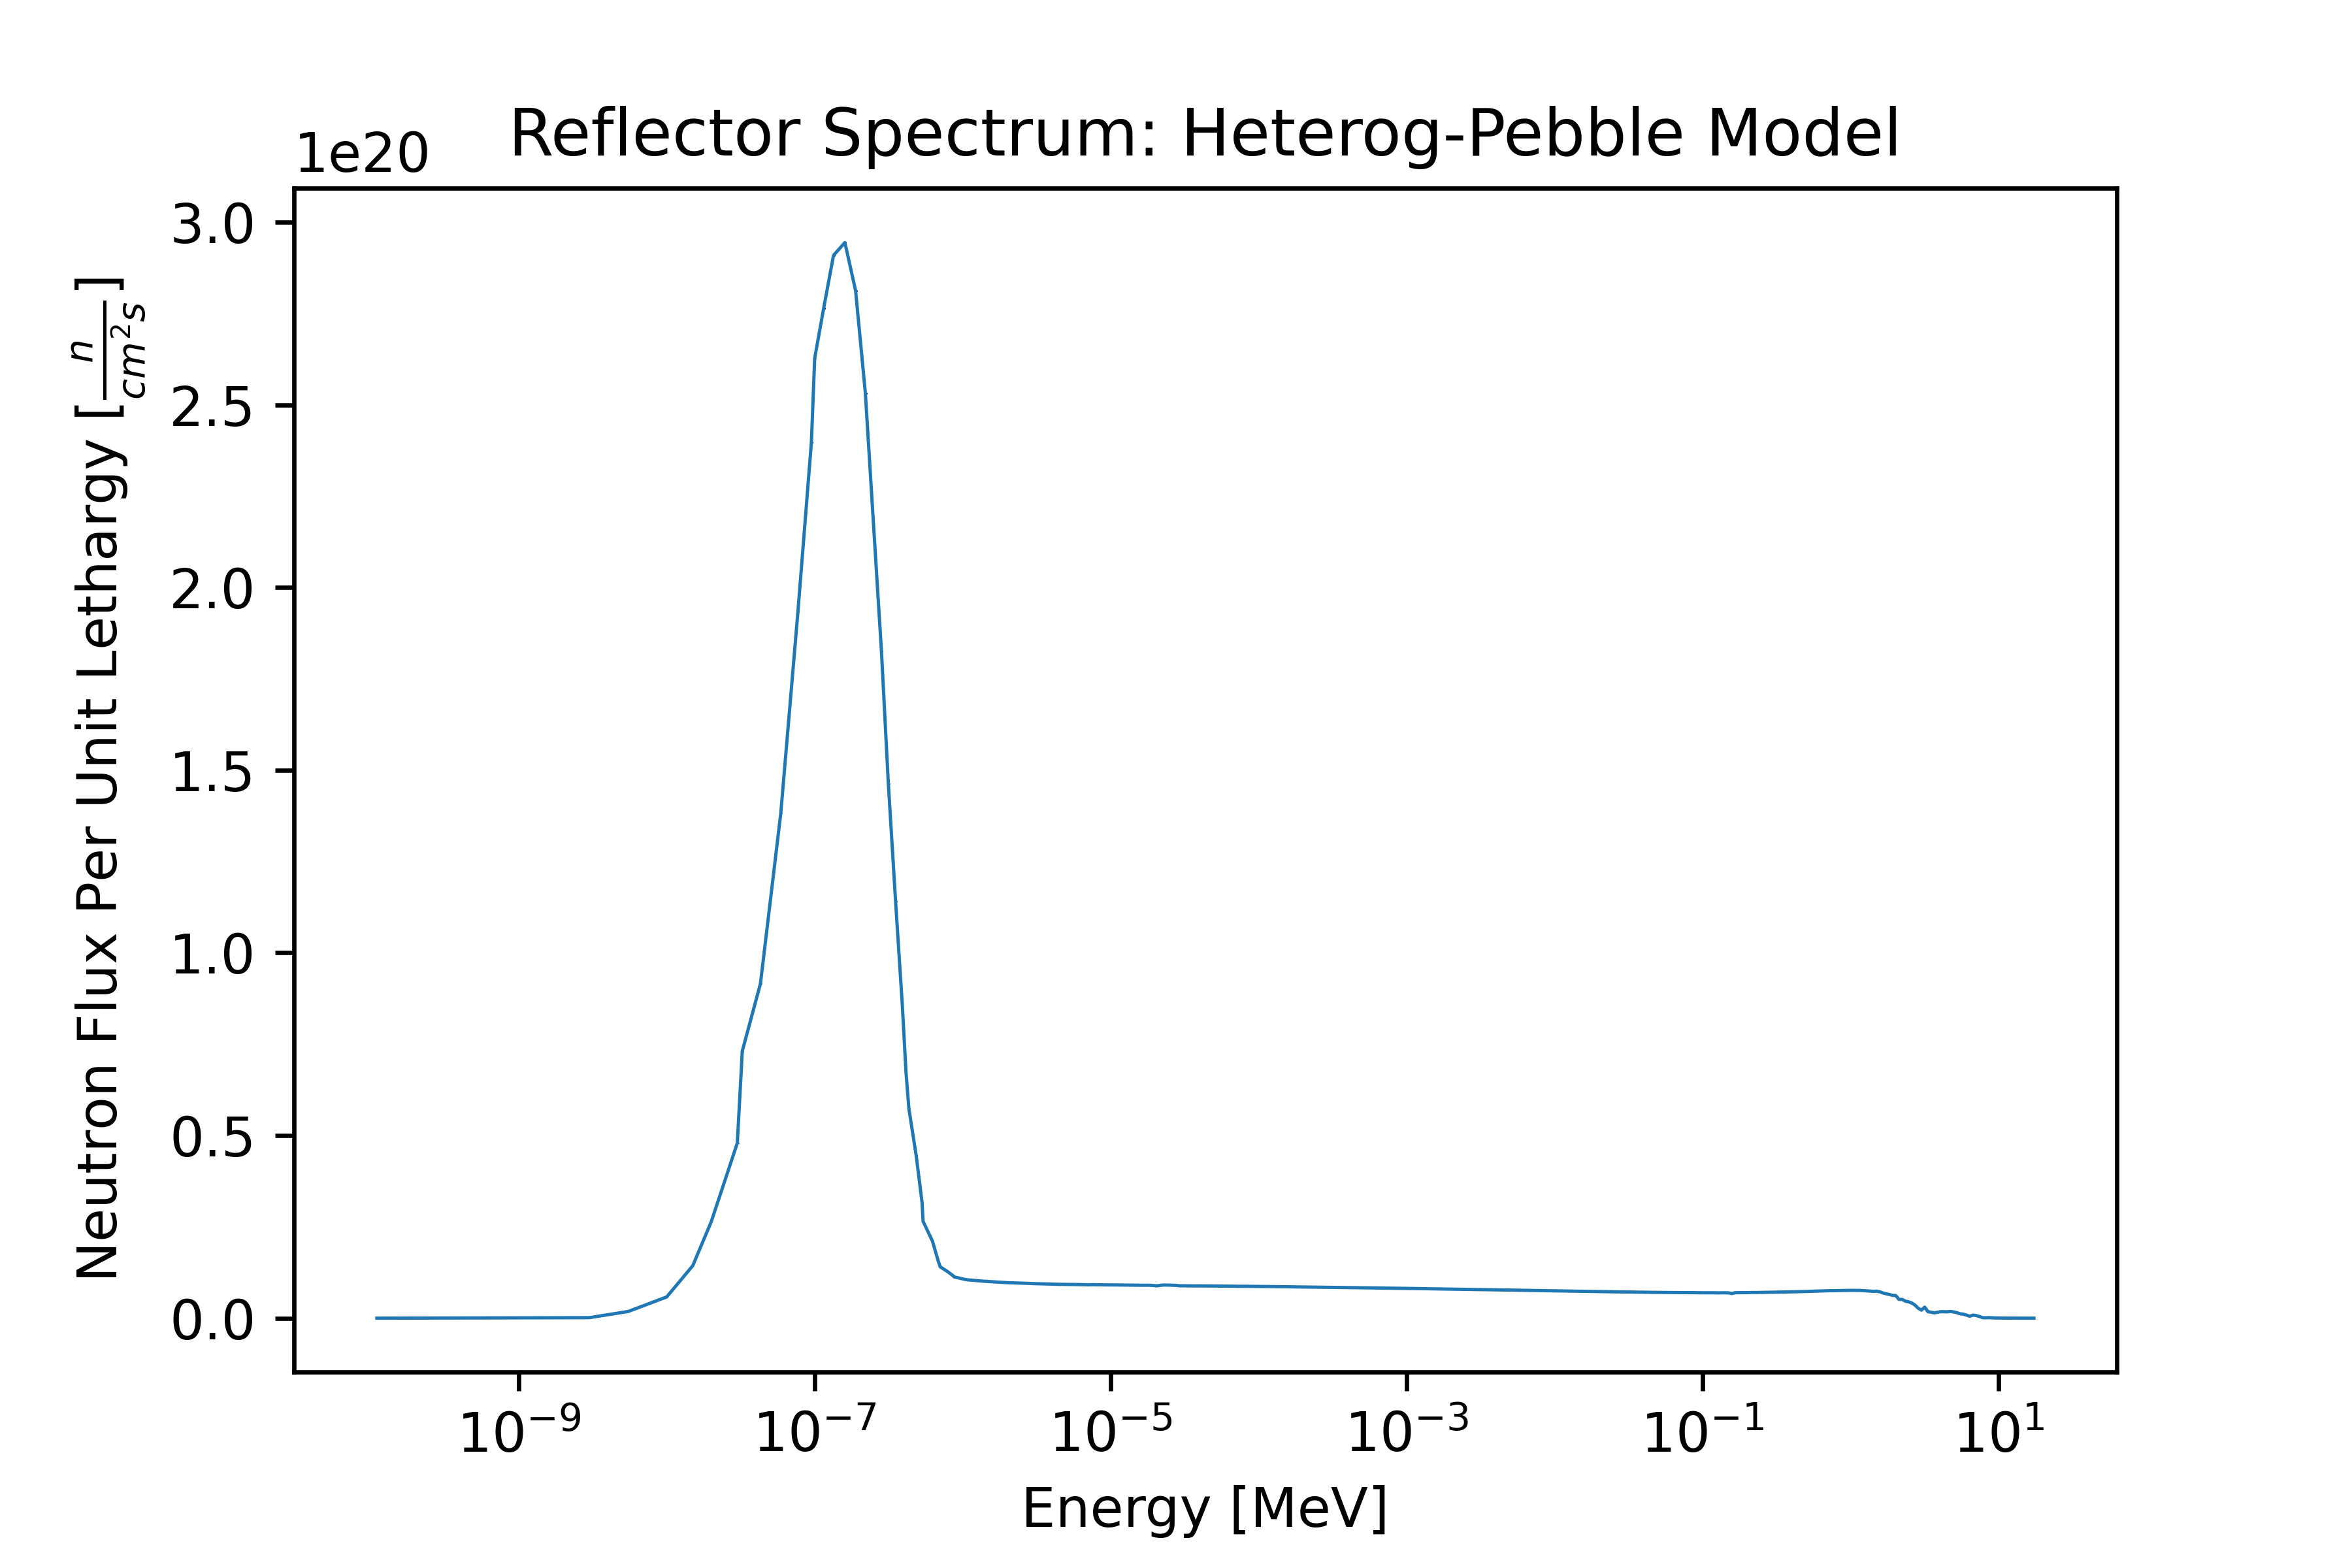
\includegraphics[width=0.95\linewidth]{figures/reflect_spec_het}
  \caption{Reflector Spectrum}
  \label{fig:het-reflec}
\end{subfigure}%
%

\caption{Lethargy Adjusted Neutron Flux Energy Spectra: Core Using Heterogenized Pebbles}
\label{fig:hom-spec}
\end{figure}